\chapter{Implementierung der automatischen Konsistenzprüfung}

Nachdem das hier vorgestellte Verfahren theoretisch erläutert wurde, wird nun eine praktische Umsetzung vorgestellt.
Dafür werden im ersten Abschnitt die technischen Rahmenbedingungen aufgeführt.
Anschließend wird jeweils die Implementierung des \emph{Matching-Algorithmus} und des \emph{Verifikations-Algorithmus} erklärt.
Im vierten Abschnitt wird die Benutzerschnittstelle des implementierten Tools vorgestellt.

\section{Implementierung der Referenzarchitektur}

Im \cref{sec:Konsistenzregeln} werden die die Konsistenzregeln mit Hilfe von einem Prolog-Dialekt eingeführt.
Dies legt nah für die Implementierung auch eine Sprache zu verwenden die auf Prolog basiert oder einfach interagieren kann.
Allerdings hat die Implementierung in Prolog einen entscheidenden Nachteil.
Für den \emph{Verifikations-Algorithmus} wird ein dreiwertiger Rückgabewert pro Regel benötigt.
Dies lässt sich mit Prolog nicht direkt abbilden.
Zudem lassen sich die Regel dank des \emph{Graph-Logik-Isomorphismus} auch direkt auf dem Graphen anwenden.
Eine weitere Anforderung an die Implementierung ist eine mögliche Integration in den bestehenden BROS-Editor FRaMED.io.
Dieser basiert auf Web-Technologien und ist in der objektorientierten Programmiersprache Kotlin entwickelt.
Aus diesem Grund wird auch Kotlin für die Entwicklung der Referenzimplementierung verwenden.
Kotlin ist als JVM-Sprache entwickelt wurden, kann aber auch zu Javascript und LLVM-Bytecode transpiliert werden.
Dadurch besitzen Kotlin Programme eine hohe Erweiterbarkeit im Bezug auf andere Laufzeitumgebungen.
Wie auch im BROS-Editor FRaMED.io wird die Transpilierung zu Javascript genutzt.
Ziel der Implementierung ist es, bestehende BPMN- und BROS-Modelle, mit Hilfe des hier vorgestellten Verfahrens, auf Konsistenz zu überprüfen.

Als Dateiformat für BPMN-Modelle wird das auf XML basierende (\emph{*.bpmn}) Format von dem BPMN-Editor bpmn.io unterstützt.
Der BPMN-Editor bpmn.io ist eine moderne und Webanwendung zum editieren von BPMN-Modellen.
Das Dateiformat enthält sowohl Strukturinformation als auch graphische Informationen.
Diese sind in zwei XML-Namespaces getrennt.
Die Struktur wird im Namespace \emph{bpmn}, und die graphische Notation im Namespace \emph{bpmndi} gespeichert.
Für die Konsistenzprüfung ist nur der Namespace \emph{bpmn} relevant.
Der Namespace \emph{bpmndi} und alle seine Kindelemente wird im folgenden ignoriert.
Zum lesen der BPMN-Datei wird der XML-Parser verwendet der von Javascript nativ bereitgestellt wird.
Von den Entwicklern von bpmn.io existiert bereits ein Parser und Validierer für BPMN-Dateien (\emph{bpmn-moddle}).
Dieser wird explizit nicht verwendet da er in Javascript geschrieben wurde und somit eine zu starke Bindung an die Platform Javascript erzeugt.
Die integrierte Validierungsfunktion für BPMŃ-Modelle wird auch nicht benötigt da eine Vorraussetzung für das benutzen des Tools die syntaktische und semantische Korrektheit der Modelle ist. 
Mit Hilfe des XML-Parsers wird das BPMN-Modell als eine Instanz des BPMN-Metamodells geladen.

Die enge Kopplung zwischen dem BROS-Editor FRaMED.io und diesem Tool legt nah auch das auf JSON basierende Format des BROS-Editors zu nutzen.
Analog zu dem BPMN-Editor, ist auch der BROS-Editor webbasiert und das Dateiformat enthält sowohl Strukturinformation als auch graphische Informationen.
Die graphischen Informationen befinden sich im Root-Objekt unter dem Schlüsselwort \emph{layer}.
Auch diese graphischen Informationen werden im weiteren ignoriert.
Zum lesen der BROS-Dateien wird der bereits existierende Parser aus dem BROS-Editor FRaMED.io genutzt.
Dieser ist in Kotlin geschrieben und benutzt den nativen JSON-Parser von Javascript.
Genau wie bei dem BPMN-Parser wird auch das BROS-Modell in eine Instanz des BROS-Metamodells geladen.

\begin{figure}
    \centering
    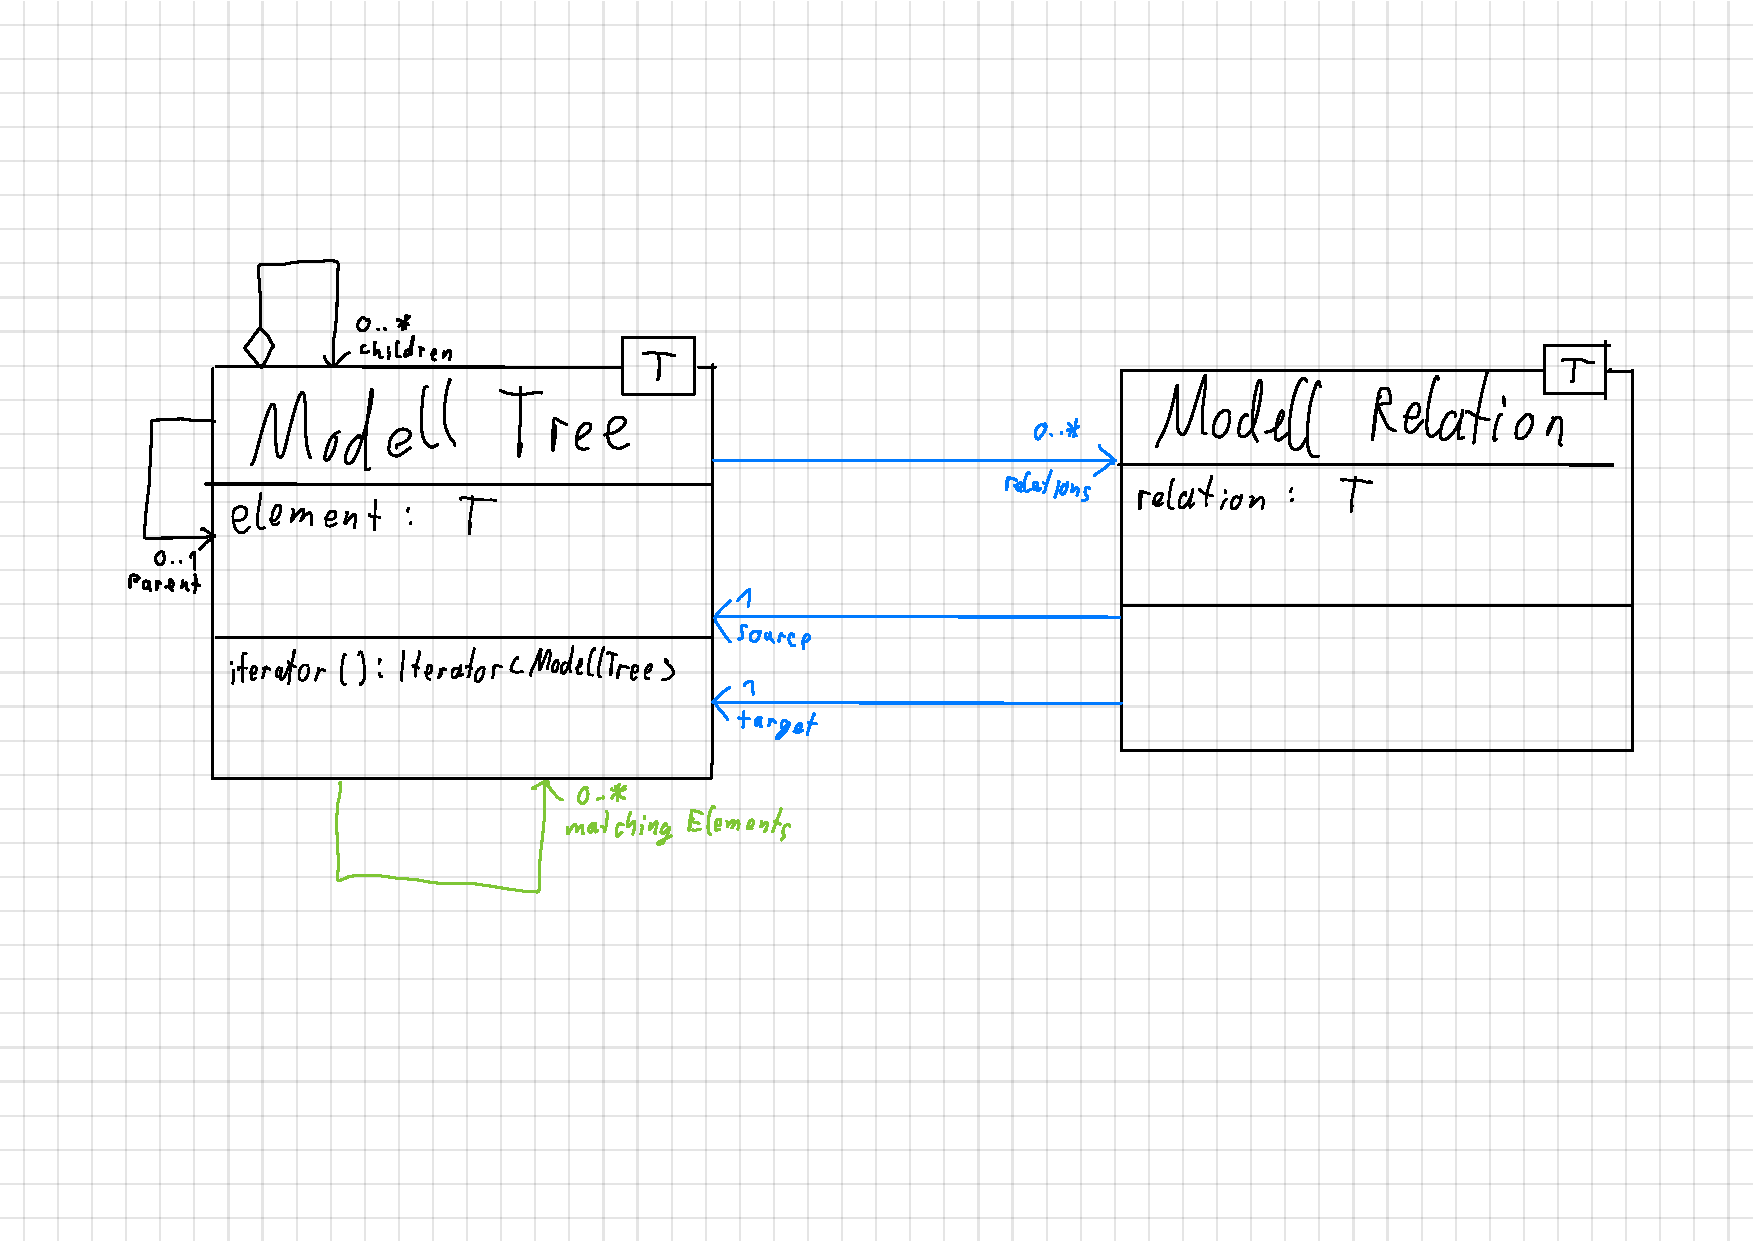
\includegraphics[width=\textwidth,keepaspectratio]{../images/UmlGraph.pdf}%
    \caption{Metamodell der Graphstruktur}%
    \label{fig:UmlGraph}
\end{figure}

Bevor der \emph{Matching-Algorithmus} und der \emph{Verifikations-Algorithmus} beginnen können, müssen beide Instanzen des Metamodells noch in die Form eines Graphen konvertiert werden.
Die Datenstruktur des Graphen basiert auf dem Metamodell aus \cref{fig:UmlGraph}.
In dieser Abbildung sind die drei Schichten des Graphen farbig hervorgehoben.
In schwarz ist die erste Schicht dargestellt.
Dabei besitzt jeder Knoten eine Liste von Kind-Knoten.
Jeder Knoten hat zusätzlich noch einen Verweis auf seinen Eltern-Knoten.
Zusätzlich besitzt jeder Knoten noch eine Referenz auf seine Metamodell Instanz mit Typannotation.
Die zweite Schicht wird in blau dargestellt un repräsentiert die Relation zwischen den Knoten.
Dabei hat jeder Knoten ein Set von Verweisen auf seine Relationen.
Die Relationen verweisen auf auf ihren Quell- und Zielknoten.
Aus die Graphrelationen besitzen eine Referenz auf ihre Metamodell Instanz mit Typannotation.
Schließlich wird die dritte Schicht, die das Matching zwischen den Modellen darstellt mit grün markiert.
Dabei handelt es sich um ein Set von Knoten.
Jeder Knoten hat zusätzlich noch eine Hilfsfunktion die einen Iterator zurückgibt.
Diese implementiert eine einfache Breitensuche um über den Graphen zu iterieren.

\section{Matching der Modelelemente}
\label{sec:matching_model_elements}

Um die Verifizierung der Modelle zu ermöglichen muss zunächst ein dazugehöriges Matching aufgebaut werden.
Um den \emph{Matching-Algorithmus} ausführen zu können muss zunächst die Orakelfunktion implementiert werden.
Dabei hat es sich als ausreichend gezeigt theoretisch miteinander kompatible Elemente anhand ihres Namens zu vergleichen.
In \cref{lst:name_matching} ist der für den Namensvergleich genutzte Algorithmus abgebildet.
Dabei werden die Namen zunächst in einzelne Wörter gesplittet und anschließend unabhängig ihrer Endung und Reihenfolge verglichen.
Um die Funktionsweise dieses Algorithmus zu verdeutlichen wird dieser Beispielhaft angewendet (Vgl. Schritt \ref{eq:name_matching_1}).
Zunächst werden beide Namen in ihre Bestandteile zerlegt (Vgl. Schritt \ref{eq:name_matching_2}) und nach der länge sortiert (Vgl. Schritt \ref{eq:name_matching_3}).
Anschließend wird für jedes Element der ersten Menge ein passendes Element in der zweiten Menge gesucht.
Die Zeichenketten müssen nicht komplett übereinstimmen.
Es ist ausrechend wenn einer der beiden Strings ohne seine Endung ein Teil des anderen Strings ist.
Um zu verhindern das ein sehr kurzer String in einem langen String erkannt wird, darf die Längenunterschied nicht größer als die Endungslänge sein.
Wenn zu jedem Element der ersten Menge ein passendes Element der zweiten Menge gefunden wird, stimmen die beiden Namen überein (Vgl. Schritt \ref{eq:name_matching_4}).

\begin{figure}
    \centering
    \begin{align}
        \text{'Aktion war erfolgreich'}\ ,&\ \text{'ErfolgreicheAktion'} \label{eq:name_matching_1}\\
        \text{\{'aktion', 'erfolgreich', 'war'\}}\ ,&\ \text{\{'aktion', 'erfolgreiche'\}} \label{eq:name_matching_2}\\
        \text{\{'aktion', 'erfolgreiche'\}}\ ,&\ \text{\{'aktion', 'erfolgreich', 'war'\}} \label{eq:name_matching_3}\\
        \text{\{'\textbf{akti}on'} \subseteq \text{'\textbf{akti}on'\}}\ ,&\ \text{\{'\textbf{erfolgreic}he'} \subseteq \text{'\textbf{erfolgrei}ch'\}} \label{eq:name_matching_4}
    \end{align}
    \caption{Anwendung des Name-Matching}
    \label{eq:name_matching}
\end{figure}

Zusätzlich zum Name-Matching müssen Regeln definiert werden auf welchen Elementen es angewendet werden muss.
Jede Regel muss das \emph{Matching} Interface implementieren.
Um diese Regeln gebündelt zu erstellen und sammeln gibt es das \emph{Context} singleton-Objekt.
Dieses bietet verschiedene Hilfsfunktionen um auf einfache Art und Weise Matching- und Verifikations-Regeln zu implementieren.
Dabei Funktion benötigt drei Parameter.
Die ersten beiden Parameter sind die Referenzen auf das BPMN- und BROS-Metamodell nach den die Graphknoten gefiltert werden soll.
Mit den Sprachfunktionen von Kotlin können diese Referenzen als generischer Parameter der Funktion übergeben werden.
Der dritte Parameter ist ein Lambda das die beiden Knoten des BPMN-Graphen und des BROS-Graphen auf einen Wahrheitswert abbildet.
Das Lambda wird nur ausgeführt wenn die Knoten zu den Filtern der ersten beiden Parameter passen.
Wenn das Lambda wahr zurück gibt werden der dritten Schicht die beiden Kanten zwischen dem BPMN- und BROS-Knoten hinzugefügt, sofern diese nicht bereits existieren.
Sonst wird das Ergebnis ignoriert, da nur Kanten zum Matching hinzugefügt werden können.
In \cref{lst:match_lane_role} ist das Matching für einer BPMN-Swimlane und einem BROS-RoleType gegeben.
Mittels der generischen Parameter werden die Graph-Knoten gefiltert und das Lambda wird nur auf den betreffenden Knoten ausgeführt. 
Im Lambda wird hier nur ein einfaches Name-Matching durchgeführt.
Die weitere Struktur wird nicht betrachtet.

\begin{lstlisting}[language=Kotlin, caption=Matching Regel von einer BPMN-SwimLane und einem BROS-RoleType, label=lst:match_lane_role]
Context.match<BpmnLane, RoleType> { lane, role ->
    matchStrings(lane.element.name, role.element.name)
}
\end{lstlisting}

Im zweiten Beispiel \cref{lst:match_gateway_event} wird das Matching zwischen einem BPMN-Gateway und einem BPMN-Event gebildet.
Hierbei ist zu beachten das die Namen der BPMN-Gateway Ausgänge nicht im Metamodell des Gateways sondern im Metamodell des weiterführenden BPMN-Flows definiert ist.
Nachdem die Knoten auf gefiltert wurden, wird überprüft ob der Name eines BPMN-SequenceFlows der an das BPMN-Gateway anschließt mit dem BROS-Event übereinstimmt.
Dafür bietet die Knoten-Klasse eine weitere Hilfsfunktion die die verbunden Relationen nach ihrem Typ gefiltert zurückgeben kann.

\begin{lstlisting}[language=Kotlin, caption=Matching Regel von einem BPMN-Gateway und einem BROS-Event, label=lst:match_gateway_event]
Context.match<BpmnGateway, Event> { bpmn, bros ->
    bpmn.relations<BpmnFlow>().any { flow ->
        flow.relation.type == BpmnFlow.Type.SEQUENCE &&
                flow.relation.name.isNotBlank() &&
                matchStrings(flow.relation.name, bros.element.desc)
    }
}
\end{lstlisting}

Das drittes Beispiel \cref{lst:match_fixpoint_event_event} zeigt die Vorteile des Fixpunkt-Algorithmus.
Diese Regel besagt das ein BPMN-Event ein äquivalentes Matching wie seine per BPMN-MessageFlow verbunden Nachbarn besitzt.
Nach dem filtern der Graphknoten, wird über alle BPMN-MessageFlows iteriert.
Ein Matching wird dann gefunden, wenn die Quelle oder das Ziel des BPMN-MessageFlows bereits ein Matching mit dem BROS-Event besitzt.
Dies ermöglicht das schreiben einfacherer Regeln.

\begin{lstlisting}[language=Kotlin, caption=Fixpunkt Matching Regel von einem BPMN-BpmnEvent und einem BROS-Event, label=lst:match_fixpoint_event_event]
Context.match<BpmnEvent, Event> { bpmn, bros ->
    bpmn.relations<BpmnFlow>().any { flow ->
        flow.relation.type == BpmnFlow.Type.MESSAGE &&
                flow.source in bros.matchingElements ||
                flow.target in bros.matchingElements
    }
}
\end{lstlisting}

Allerdings kann es auch vorkommen das trotz dieser Regeln ein Matching zwischen zwei Elementen nicht gefunden wird oder auch fälschlicher Weise gefunden wirde.
Für diesen Fall hat der Modellierer die Möglichkeit ein sogenanntes \emph{Predefined-Matching} hinzuzufügen.
Damit lässt sich ein Matching zwischen Elementen hinzufügen oder auch entfernen.
Das \emph{Predefined-Matching} wird in jeder Iteration des Fixpunkt-Algorithmus, nachdem die Regeln auf den gesamten Graphen angewendet wurden ausgeführt.
Durch das entfernen von Kanten aus dem Graphen ist es bei einem Fixpunkt-Algorithmus theoretisch möglich in einen nicht terminierenden Zustand überzugehen.
Da aber in jeder Iteration, vor dem überprüfen auf Änderungen in der dritten Schicht, ein konstante Kantenmenge entfernt wird, reduziert dies nur den vollständigen Graphen auf einen Graphen ohne diese Kantenmenge.
Dabei bleibt die dritte Schicht, am Ende jeder Iteration, monoton wachsend. 

\section{Implementierung der Konsistenzregeln}
\label{sec:implementaion_consistency_rules}

Nach dem Aufbau des Matching in der dritten Schicht, kann der \emph{Verifikations-Algorithmus} arbeiten.
Für das implementieren der Regeln stellt das Context Objekt zwei Hilfsfunktionen bereit.
Dies sind die Funktionen \emph{verifyBpmn} und \emph{verifyBros} welche jeweils zwei Parameter benötigen.
Der erste Parameter ist der Filter des Graph-Knoten.
Dieser stellt die Vorbedingung aus der Implikation in \cref{sec:Konsistenzregeln} dar.
Der zweite Parameter ist ein Lambda das den gefilterten Graphknoten auf ein Konsistenzmeldung abbildet.
Damit wird die Konsequenz der Implikation dargestellt.
Neben einer positiven und einer negativen Konsistenzmeldung kann auch kann auch ein \emph{null} Wert zurückgegeben werden.
Ein \emph{null} Wert bedeutet, das die Regel nicht anwendbar ist und das Ergebnis daher ignoriert werden soll.
Damit wird die unter \cref{sec:Konsistenzregeln} beschriebende Dreiwertigkeit umgesetzt.

Um dies zu veranschaulichen werden nachfolgend die Konsistenzregeln 2, 3 und 5 in ihre Kotlin-Implementierung überführt.

\textbf{Regel 2} ist die einfachste zu implementierende Regel.
Sie besagt das zu jeder BPMN-Swimlane ein passender BROS-RoleType existieren muss.
Die zweite Regel ist auf dem BPMN-Graphen basiert und filtert in der Vorbedingung nach der BPMN-Swimlane.
Dies wird mit dem Metamodell dargestellt und als erster generischer Parameter der Hilfsfunktion \emph{verifyBpmn} übergeben.
In der Konsequenz der Implikation wird nach einem BROS-RoleType gesucht das ein Matching mit der BPMN-Swimlane aufweist.
Bei der Kotlin-Implementierung wird dies aus der anderen Richtung betrachtet.
Da alle Elemente die ein Matching mit der BPMN-Swimlane habe bekannt sind, wird unter diesen Elementen ein BROS-RoleType gesucht.
Sobald eines gefunden ist wird eine positive Konsistenzmeldung zurückgegeben.
Um die Rückmeldung an den Modellierer zu verbessern wird der Konsistenzmeldung noch eine textuelle Beschreibung und eine Referenz auf den Knoten des BROS-Graphen auf den die Regel erfolgreich angewendet wurde hinzugefügt.
Die Referenz zu dem Knoten des BPMN-Graphen wird automatisch von der Hilfsfunktion hinzugefügt.
Sollte kein Element gefunden werden, wird eine negative Konsistenzmeldung zurückgeben.
Auch diese Meldung beinhaltet eine textuelle Beschreibung der Fehlerursache.
Die Referenzangabe zu einem weiteren Knoten ist optional und kann, wenn die Information nicht verfügbar oder für die Auswertung des Modellierers nicht hilfreich ist, weggelassen werden.

\begin{lstlisting}[language=Kotlin, caption=Implementierung von Regel 2, label=lst:implementation_rule_2]
Context.verifyBpmn<BpmnLane> { bpmn ->
    for (match in bpmn.matchingElements) {
        val roleType = match.model<RoleType>() ?: continue
        return@verifyBpmn Result.match("...", bros = match)
    }
    Result.error("...")
}
\end{lstlisting}

Die \textbf{Regel 3} ist ähnlich aufgebaut wie Regel 2.
In der Regel 3 wir überprüft das zu jedem BPMN-TerminationEvent ein passendes BROS-ReturnEvent existiert.
Genau wie die Regel 2 basiert sie auf dem BPMN-Graphen.
Allerdings ist ein BPMN-TerminationEvent im BPMN-Metamodell ein normales BPMN-Event das zusätzlich ein Attribut TerminationEvent besitzt.
Hierfür ist die Dreiwertigkeit des Rückgabewertes wichtig.
Zunächst wird in der Vorbedingung nach einem BPMN-Event gefiltert.
Anschließend wird jedes gefundene BPMN-Element überprüft, ob es auch ein BPMN-TerminationEvent ist.
Sollte dies nicht der Fall sein wird das Lambda mit dem Rückgabewert null beendet.
Damit wird die Ausführung der Regel komplett ignoriert, genau wie bei dem generischen Filterargument.
Wenn nun ein BPMN-TerminationEvent gefunden ist, kann, analog zu Regel 2, in der dritten Schicht nach einem BROS-ReturnEvent gesucht werden.
Der Rückgabewert null ermöglicht auch komplexere Vorbedingungen leicht zu überprüfen.

\begin{lstlisting}[language=Kotlin, caption=Implementierung von Regel 3, label=lst:implementation_rule_3]
Context.verifyBpmn<BpmnEvent> { bpmn ->
    if (!bpmn.element.terminationEvent) return@verifyBpmn null

    for (match in bpmn.matchingElements) {
        val returnEvent = match.model<ReturnEvent>() ?: continue
        return@verifyBpmn Result.match("...", bros = match)
    }
    Result.error("...")
}
\end{lstlisting}

\textbf{Regel 5} gehört zu den komplexeren Regeln.
Sie überprüft das zu jedem BPMN-StartEvent ein passendes BROS-Event existiert.
Zusätzlich müssen beide Events auch zueinander passende Elemente erstellen bzw. starten.
In der Vorbedingung wird überprüft, das das BPMN-Element eine BPMN-Event ist, keine BPMN-TerminationEvent ist und der Typ des BPMN-Events ein BPMN-StartEvent ist.
Dabei wird erneut der null Rückgabewert genutzt.
Anschließend wird in der dritten Schicht nach einem BROS-Event gesucht.
Bei dem BROS-Event wird in der zweiten Schicht nach einer BROS-CreateRelationship gesucht.
Diese verbindet ein BROS-Event mit dem von ihm erzeugten Element.
Nun wird überprüft ob das Ziel der BROS-CreateRelationship sich mit in der dritten Schicht des Elternelementes des BPMN-StartEvents befindet.
Ein BPMN-StartEvent beginnt seine BPMN-Swimlane, die auch sein Elternelement ist.
Wenn dieses Überprüfung erfolgreich ist wird eine positive Konsistenzmeldung zurückgegeben, sonst eine negative.
Beide Konsistenzmeldung haben neben der textuellen Beschreibung auch eine Referenz auf das BPMN-Event.
Sollte kein passendes BPMN-Event gefunden werden, wird auch eine negative Konsistenzmeldung zurückgegeben, allerdings ohne eine Referenz auf ein BROS-Event.
\textit{TODO: mehrere CreateRelationsips}

\begin{lstlisting}[language=Kotlin, caption=Implementierung von Regel 5, label=lst:implementation_rule_5]
verifyBpmn<BpmnEvent> { bpmn ->
    if (
        bpmn.element.terminationEvent || 
        bpmn.element.type != BpmnEvent.Type.START
    ) return@verifyBpmn null

    for (match in bpmn.matchingElements) {
        val event = match.model<Event>() ?: continue
        val container = bpmn.container()?.second ?: continue

        val createsElement = match.relations<CreateRelationship>()
                .firstOrNull()
                ?.target as? ModelTree<ModelElement<*>> ?: continue

        if (createsElement in container.second.matchingElements) {
            return@verifyBpmn Result.match("...", bros = match)
        } else {
            return@verifyBpmn Result.error("...", bros = match)
        }
    }
    Result.error("...")
}
\end{lstlisting}

\section{Benutzerinterface}

Da das entwickelte Tool eine Webanwendung ist kann es in allen moderneren Browsern benutzt werden die Javascript aktiviert haben.
Das Tool hat ein zweistufiges Interface.
Als erster Schritt müssen die Quelldateien der zu überprüfenden Modelle geladen werden.
Dazu können die Dateien einfach per Drag'n'Drop in das Tool geladen werden.
Das Tool erkennt den Inhalt unabhängig des Namens und läd die entsprechende Datei.
Alternativ kann eine manuelle Dateiauswahl genutzt werden oder der Inhalt der Datei in das entsprechende Textfeld kopiert werden.
Sobald jeweils ein valides BPMN- und BROS-Modell geladen wurden, wird die Konsistenzprüfung automatisch gestartet.

Die Ergebnisse der Konsistenzprüfung werden unterhalb der Eingabemaske angezeigt.
Zunächst werden statistische Informationen zu den geladen Modellen, des Matchings und der Validierung angezeigt.
Diese sind in drei Abschnitte unterteilt.
\begin{itemize}
    \item \textbf{Verification stats:} Informationen zu der aktuellen Verifikation.
    \begin{itemize}
        \item \emph{Successful checks (x of y):} Anzahl der \emph{x} positiven Konsistenzmeldung von allen \emph{y} Konsistenzmeldung. 
        \item \emph{Errors (x of y):} Anzahl der \emph{x} negativen Konsistenzmeldung von allen \emph{y} Konsistenzmeldung. 
        \item \emph{Coverage (x\%):} Prozentualle Anzeige \emph{x} der \emph{Successful checks}.
        \item \emph{Fixed point matching rounds (x):} Anzahl der durchgeführten Matching Runden \emph{x} aufgrund des Fixpunkt-Algorithmus. Mögliche Werte von \emph{x} sind:
        \begin{itemize}
            \item \emph{1:} Es wurde kein Matching gefunden.
            \item \emph{2:} Es wurde ein Matching gefunden. Es gibt kein Matching was auf ein anderes Matching aufbaut.
            \item \emph{3-5:} Es wurde ein Matching gefunden. Es gibt ein oder mehrere Matchings die auf andere Matching aufbauen.
            \item \emph{>=6:} Es wurde ein Matching gefunden. Es ist möglich das ein kaskadieren Effekt eingetreten ist und ein zu großes Matching aufgebaut wurde. Das Matching sollte von dem Modellierer überprüft werden.
        \end{itemize}
    \end{itemize}
    \item \textbf{BPMN/BROS matching stats} Informationen zu dem Matching aus Sicht des BPMN bzw. BROS Modelles.
    \begin{itemize}
        \item \emph{Matched elements (x of y):} Anzahl der \emph{x} Elemente mit gefundenem Matching von allen \emph{y} Elemente.
        \item \emph{Unmatched elements (x of y):} Anzahl der \emph{x} Elemente ohne gefundenem Matching von allen \emph{y} Elemente.
        \item \emph{Multiple matches (x):} Anzahl der \emph{x} Elemente die mit mehreren Elementen ein Matching haben. 
        \item \emph{Coverage (x\%):} Prozentualle Anzeige \emph{x} der \emph{Matched elements}.
    \end{itemize}
\end{itemize}

Unterhalb dieser Statistiken befindet sich die Liste der Validierungsergebnisse.
Mit hilfe der Tableiste kann zusätzlich das BPMN- oder BROS-Matching oder auch das geladene Predefined-Matching angezeigt werden.
Jeder Eintrag der Liste hat den gleichen Aufbau.
Auf der linken Seite de Eintrages ist farblich der Typ markiert. Je nach Tab gibt es unterschiedliche Farbkodierungen.
Im Hauptteil des Eintrages sind drei Textfelder.
Diese sind das BPMN-Element, das BROS-Element und die textuelle Beschreibung des Eintrages.
Zusätzlich ist noch ein viertes Textfeld vorhanden das den Namen der Regel angibt, die diesen Eintrag erstellt hat.
Mit einem klick auf das Textfeld des BPMN- oder BROS-Elementes kann direkt ein PredefinedMatching erstellt oder gelöscht werden.
Die Verifizierungsergebnisse haben die Farbkodierungen grün (positive Konsistenzmeldung) und rot (negative Konsistenzmeldung).
Die Matching Ergebnisse sind blau (Matching für dieses Element gefunden) und gelb (keine Matching für dieses Element gefunden) markiert.
Da sich nicht alle Elemente eines Modelles auf das andere Abbilden lassen, ist ein Fehlendes Matching meißt kein Fehler.
Genauso ist das vorhanden sein eines Matchings nicht immer korrekt, da das Matching auf die Namen angewiesen ist. 
Aus diesem Grund ist die Farbkodierungen des Matchings schwächer als die der Verifizierung.
Ein bestehendes PredefinedMatching kann auch im Tab PredefinedMatching mit dem Löschen Button oben rechts in jedem Eintrag entfernt werden.
